\EnableTitleSlide
\section{Grundlagen}

\begin{frame}{Rewrite Rules}
    \textbf{Benutzen einer Rewrite Rule}: \vspace{5mm}

    \begin{tcbitemize}[raster equal height=rows, raster columns=3,
        raster every box/.style={size=small,valign=center,halign=center,colframe=white,colback=white}]
        \tcbitem
        \tcbitem {\Large\color{red-500} $a \cdot 0 \Leftrightarrow 0$ }
        \tcbitem 
    \end{tcbitemize}\vspace{5mm}
    \pause

    \begin{tcbitemize}[raster equal height=rows, raster columns=3,
        raster every box/.style={size=small,valign=center,halign=center,colframe=white,colback=white}]
        \tcbitem {\Large $x + \eqnmarkbox[red]{node5}{y \cdot 0}$ } 
        \annotate[yshift=-1.5em]{below,right}{node5}{Anwenden der Regel} 
    \tcbitem\begin{tikzpicture}
        \draw[line width=10mm, -{Stealth[length=4mm, open, round]}, black, thick] (0,0) -- (2,0);
    \end{tikzpicture}
        \tcbitem {\Large $x$}
    \end{tcbitemize}
\end{frame}

\begin{frame}{Naiver Algorithmus}

    \begin{algorithm}[H]
        \caption{Naiver Algorithmus zur Optimierung von Ausdrücken}\label{alg:ausdruck1}
        \begin{algorithmic}
          \Function{optimize\_expression}{expression}
          \State rules $\gets$ [\ldots]
          
          \While{old\_expression $\neq$ expression}
            \State old\_expression $\gets$ expression
      
            \For{rule in rules}
              \If{match(expression, rule)}
              \State apply(expression, rule)
              \EndIf
            \EndFor
          \EndWhile
      
          \State \Return expression
          \EndFunction
        \end{algorithmic}
      \end{algorithm}
   
\end{frame}

\begin{frame}{Phase Ordering Problem}
    \begin{center}
        \textbf{Welche Regel soll zuerst angewendet werden?}
    \end{center}\vspace{5mm}

    \begin{center}
        {\Large $\left(\eqnmarkbox[red]{node5}{\frac{x \cdot 2}{2}} + x \cdot \frac{y - 3 + 3 + z \cdot 0}{x}\right)^2$ }\vspace{7mm}
    \end{center}

    \begin{center}
        \textbf{Mögliche Resultate:}
    \end{center}\vspace{2mm}

    \begin{tcbitemize}[raster equal height=rows, raster columns=2,
        raster every box/.style={size=small,valign=center,halign=center,colframe=white,colback=white}]
        \tcbitem {\Large $\eqnmarkbox[red]{node5}{\frac{x \ll 1}{2}}$}
        \tcbitem {\Large $\eqnmarkbox[red]{node5}{x}$}
    \end{tcbitemize}
\end{frame}

\begin{frame}{Lösung}
    \textbf{Speichern aller möglichen Ausdrücke in Liste}: \vspace{5mm}

    \begin{tcolorbox}[title=ExprList, center title]
        $\left(\eqnmarkbox[red]{node5}{\frac{x \cdot 2}{2}} + x \cdot \frac{y - 3 + 3 + z \cdot 0}{x}\right)^2$,
        $\left(\eqnmarkbox[red]{node5}{\frac{x \ll 1}{2}} + x \cdot \frac{y - 3 + 3 + z \cdot 0}{x}\right)^2$,
        $\left(\eqnmarkbox[red]{node5}{x} + x \cdot \frac{y - 3 + 3 + z \cdot 0}{x}\right)^2$
    \end{tcolorbox}
\end{frame}

\begin{frame}{Verbesserung}
    \textbf{Sharing und Klassen}: \vspace{5mm}

    {\captionsetup[figure]{oneside,margin={0.4cm,0cm}}
\begin{minipage}[c]{0.49\textwidth}
    \begin{figure}[H]
        \centering
        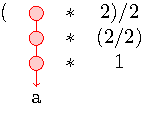
\includegraphics[scale=1.6]{utils/sharing.pdf}
        \caption{Sharing bei einer Liste von Ausdrücken}
        \label{fig:sharing}
    \end{figure}
    \end{minipage}
    \begin{minipage}[c]{0.49\textwidth}
    \begin{figure}[H]
        \centering
        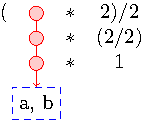
\includegraphics[scale=1.6]{utils/classes.pdf}
        \caption{Kombination aus Sharing und Klassen bei einer Liste von Ausdrücken}
        \label{fig:classes}
    \end{figure}
\end{minipage}}
\end{frame}

\begin{frame}{E-Graphs (1)}
    \begin{figure}[H]
        \centering
        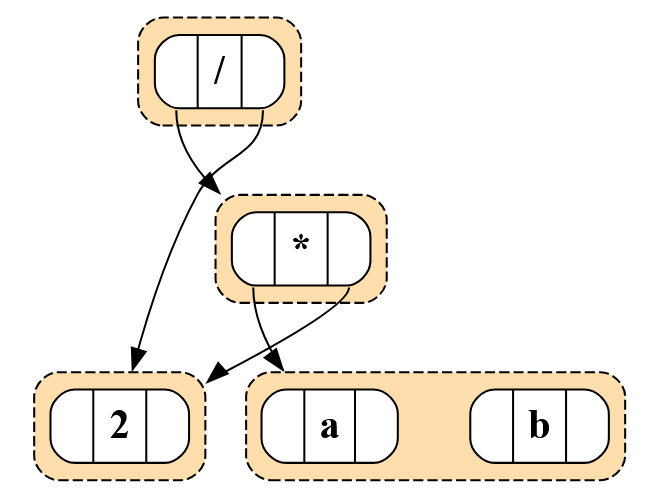
\includegraphics[scale=0.4]{utils/egraph_exp.png}
        \caption{Beispiel eines E-Graphs, der die Ausdrücke $(a \cdot 2) / 2$ und $(b \cdot 2) / 2$ enthält}
        \label{fig:egraphexp}
    \end{figure}
\end{frame}

\begin{frame}{E-Graphs (2)}
Der \textit{E-Graph} als Datenstruktur für Abbildung~\ref{fig:egraphexp}: \vspace{5mm}

\begin{itemize}
  \item $\mathbf{U}$: \{ID1\}, \{ID2\}, \{ID3\}, \{ID4, ID5\} 
  \item $\mathbf{M}$: $ID1 \rightarrow EClass(\ldots)$, $ID2 \rightarrow EClass(\ldots)$, $ID3 \rightarrow EClass(\ldots)$, \ldots 
  \item $\mathbf{H}$: $/ \rightarrow ID1$, $* \rightarrow ID2$, $2 \rightarrow ID3$, $a \rightarrow ID4$, $b \rightarrow ID5$
\end{itemize}
\end{frame}

\begin{frame}{Equality Saturation}
    \begin{algorithm}[H]
        \caption{Traditioneller Equality Saturation Workflow nach~\cite{2021-egg}}\label{alg:eqsat}
        \begin{algorithmic}
          \Function{eqsat}{expr, rewrites}
          \State egraph $\gets$ initial\_egraph(expr)
          
          \While{$\mathbf{not}$ egraph.is\_saturated\_or\_timeout()}
            
            \For{rw in rewrites}
              \For{(subst, eclass) $\mathbf{in}$ egraph.ematch(rw.lhs)}
                \State  eclass2 $\gets$ egraph.add(rw.rhs.subst(subst))
                \State egraph.merge(eclass, eclass2)
              \EndFor 
            \EndFor
          \EndWhile
      
          \State \Return egraph.extract\_best()
          \EndFunction
        \end{algorithmic}
    \end{algorithm}
\end{frame}

% \begin{frame}{Komplexe Zahlen $\mathbb{C}$}    
%     \begin{columns}[c]
%         \column{0.4\textwidth}
%             \begin{itemize}
%                 %\item Zahlen der Form $c=a+bi$ mit $a,b \in \mathbb{R}$
%                 \item $\mathbb{C} := \{a+ bi: a, b \in \mathbb{R}\}$
%                 \begin{itemize}
%                     \item Realteil $Re(c)=a$
%                     \item Imaginärteil $Im(c)=b$
%                     \item Imaginäre Einheit $i$: $i^2 := -1$
%                 \end{itemize}
%                 \item $|c| = \sqrt{a^2+b^2}$
%                 \item $\mathbb{N} \subset \mathbb{Z} \subset \mathbb{Q} \subset \mathbb{R} \subset \mathbb{C}$
%             \end{itemize}
%             \column{0.3\textwidth}
%             \begin{exampleblock}{Beispiel}
%                 \vspace{-0.45cm}
%                 \begin{align*}
%                     c_1&=3 + 4i \\[0.2cm]
%                     |c_1|&=\sqrt{3^2+4^2}\\ 
%                     &=\sqrt{25} \\
%                     &=5
%                 \end{align*}
%             \end{exampleblock}
%             \column{0.2\textwidth}
%     \end{columns}
% \end{frame}

% % Komplexe Ebene
% \begin{frame}{Komplexe Ebene}    
%     \begin{columns}[c]
%         \column{.45\textwidth}
%             \begin{itemize}
%                 \item "`Gaußsche Zahlenebene"'
%                 \item Komplexen Zahl $c=a+bi$ als kartesische Koordinate $(a,b) \in \mathbb{R}^2$
%                 \item x-Achse codiert den Realteil $Re(c)$
%                 \item y-Achse codiert den Imaginärteil $Im(c)$
%             \end{itemize}
%             \onslide<2->{
%             \begin{exampleblock}{Beispiel}
%                 $c_{{\scriptscriptstyle \color{red}{\text{P1}}}}=-1.2 + 1i$
%             \end{exampleblock}
%             }
%         \column{.45\textwidth}
%             % \only<1>{\vspace{0.18cm}
%             % \includegraphics[scale=0.75]{utils/komplexe_Ebene/ebene_plain.pdf}}
%             % \only<2->{
%             % \includegraphics[scale=0.75]{utils/komplexe_Ebene/ebene_plain_example.pdf}}
%     \end{columns}
% \end{frame}



% % Folgen
% %\begin{frame}{Folgen}
% %    \begin{itemize}
% %        \item Durch Muster oder Regeln definierte (unendliche) Aufzählung von Zahlen
% %        \item Folgeglieder $(a_n)_{n \in \mathbb{N}}$
% %        \item Definierbar über Reihen, Algorithmen, Rekursionsvorschriften $\dots$
% %        \item Beschränktheit nach oben durch $k$ $\Leftrightarrow$ $\forall n \in \mathbb{N} : a_n \leq k$ 
% %    \end{itemize}
% %    \vspace{0.2cm}
% %    \begin{block}{Beispiel: Fibonaccifolge}
% %        $f_{n}=f_{n-1}+f_{n-2}$ mit $f_1=f_2=1$
% %    \end{block}
% %    \begin{exampleblock}{Ergebnis: $(f_n)_{n \in \mathbb{N}}$}
% %        $1, 1, 2, 3, 5, 8, 13, 21, 34, 55, 89, 144, 233, 377, 610, 987, 1597, 2584 \dots$
% %    \end{exampleblock}
% %\end{frame}


% % Mandelbrot-Menge
% \begin{frame}{Mandelbrot-Menge}
%     \begin{columns}[c]
%         \column{.6\textwidth}
%             \begin{itemize}
%                 \item $ \color<2>{lightgray}\mathbb{M} :=\{ c \in \mathbb{C} \ | \ \color<1,2,3>{black}{z_{n+1} = z^{2}_{n} + c} \;\; \color<2>{lightgray}\textrm{ist beschränkt} \}$ mit $z_0=0$
%                 \begin{itemize}
%                     \item $(z_n)_{n \in \mathbb{N}}$ ist rekursiv definierte Folge
%                 \end{itemize}
%                 \item $c \in \mathbb{M}$ als schwarze Punkte in der komplexen Zahlenebene markiert 
%                 \item Beschränktheit in Praxis nur nach $m \in \mathbb{N}_0$ Iterationen abschätzbar:
%             \end{itemize}\vspace{0.25cm}
%             \begin{block}{\centering Beschränktheitskriterium}
%                 %Ist ein Folgenglied weiter als $2$ vom Ursprung entfernt, ist $c$ nicht Teil der Mandelbrotmenge \\
%                 \centering
%                 $\exists n \leq m: |z_n| > 2 \Longrightarrow c \notin \mathbb{M}$
%             \end{block}
%         \column{.40\textwidth}
%             % \includegraphics[scale=0.34]{../Code/Mandelbrot_axes/Fig1_axis_big.jpg}
% \end{columns}
% \end{frame}